% gof_brdf_preprint.tex
% Manuscrito derivado do science_template.tex (AAAS, v1.1); renomeado conforme exige o readme.txt do template.
% Versao v0 (preprint para revisao interna). Pacotes extras ao template estao marcados [preprint] e
% devem ser removidos ou revistos numa eventual submissao a um periodico da familia Science.

%%%%%%%%%%%%%%%% PREAMBULO %%%%%%%%%%%%%%%

\documentclass[12pt]{article}

\usepackage[T1]{fontenc}                 % [preprint] hifenizacao correta de palavras acentuadas
\usepackage[brazilian]{babel}            % [preprint] texto em portugues
\usepackage{amsmath}                     % [preprint] equacoes; carregado antes do newtx
\usepackage{newtxtext,newtxmath}
\usepackage{graphicx}
\usepackage[letterpaper,margin=1in]{geometry}
\usepackage{booktabs}                    % [preprint] tabelas
\usepackage{array}                       % [preprint] colunas alinhadas a esquerda
\usepackage{xcolor}                      % [preprint] marcacoes de revisao
\usepackage{lineno}                      % [preprint] numeracao de linhas para a revisao
\linespread{1.5}
\frenchspacing

\renewenvironment{abstract}
	{\quotation}
	{\endquotation}
\date{}
\renewcommand\refname{Referências e notas}

\makeatletter
\renewcommand{\fnum@figure}{\textbf{Figura \thefigure}}
\renewcommand{\fnum@table}{\textbf{Tabela \thetable}}
\makeatother

\usepackage{scicite}
\usepackage{url}
\usepackage[hidelinks]{hyperref}         % [preprint] links de DOI e referencias cruzadas

%%%%%%%%%%%% COMANDOS PROPRIOS %%%%%%%%%%%%

\newcommand{\revisar}[1]{\textcolor{red}{[#1]}}
\makeatletter
\newcommand{\inputtab}[1]{\@@input #1 } % \input expansivel, necessario dentro de tabular
\makeatother
\newcommand{\bn}{\mathbf{n}}
\newcommand{\br}{\mathbf{r}}
\newcommand{\bs}{\mathbf{s}}
\newcommand{\bc}{\mathbf{c}}
\newcommand{\dB}{\,dB}

%%%%%%%%%%%%%%%% TITULO E AUTORES %%%%%%%%%%%%%%%%

\def\scititle{
	Sombreamento especular em \emph{Gaussian Opacity Fields}: integração sem alterar o rasterizador e avaliação controlada em objetos brilhantes
}
\title{\bfseries \boldmath \scititle}

\author{
	\revisar{Autor(a)~1}$^{1\ast}$,
	\revisar{Autor(a)~2}$^{1}$\and
	\small$^{1}$\revisar{Departamento, Universidade Federal Fluminense, Niterói, Brasil (confirmar)}.\and
	\small$^\ast$Autor(a) correspondente. E-mail: \revisar{preencher}\and
	\small Versão v0 --- \emph{preprint} para revisão interna; não citar.
}

\begin{document}

\maketitle
\linenumbers

\begin{abstract} \bfseries \boldmath
Métodos de reconstrução baseados em Gaussianas 3D representam a aparência dependente da vista por harmônicos esféricos de baixa ordem, o que borra reflexos especulares e mistura iluminação com material.
O \emph{Gaussian Opacity Fields} (GOF) acrescenta geometria contínua e extração de malha, mas herda esse modelo de cor; o GaussianShader introduz uma função de sombreamento com tom especular, rugosidade e mapa de ambiente, mas sem o campo de opacidade do GOF.
Investigamos se esse sombreamento pode ser acoplado ao GOF sem modificar o rasterizador e quanto isso altera qualidade e custo.
A cor de cada Gaussiana é calculada fora do rasterizador (difuso mais Fresnel--Schlick vezes luz pré-filtrada) e entregue pelo caminho de cor pré-computada, que já é diferenciável; com tom especular nulo e Fresnel desligado, a imagem coincide com a do GOF (diferença máxima abaixo de $10^{-5}$), o que torna a ablação controlada.
Na cena real Truck, o termo especular eleva o PSNR em 0,41\,dB (IC 95\%: 0,29 a 0,53; 28 de 32 vistas).
Em três objetos brilhantes do NeRO, a configuração herdada do Truck ganha 2,0 a 2,5\,dB sobre o GOF em dois objetos e nada no mais espelhado; ajustando três hiperparâmetros, o método empata com o GaussianShader nesse objeto ($-$0,01\,dB) e o supera nos outros dois (+1,37 e +0,58\,dB), gastando de 2,7 a 4,0 vezes menos energia de GPU e metade da memória.
Os números vêm de uma semente por configuração, e o ajuste foi escolhido em um dos objetos de teste; repetir sementes e separar os ajustes são os próximos passos.
\end{abstract}

%%%%%%%%%%%%%%%%%%%%%%%%%%%%%%%%%%%%%%%%%%%%%%%%%%%%%%%%%%%%%%%%%%%%%%%%%%%%%%%%
\section{Introdução}

A síntese de novas vistas e a reconstrução 3D a partir de fotografias calibradas passaram, em poucos anos, de representações implícitas por redes neurais~\cite{mildenhall2020nerf} para representações explícitas por Gaussianas 3D rasterizadas em tempo real~\cite{kerbl2023gaussian,bao2025survey}.
Nessas representações, a cor de cada Gaussiana é uma função da direção de observação escrita em harmônicos esféricos (SH) de grau baixo.
Essa escolha é eficiente e suficiente para superfícies foscas, mas tem duas consequências conhecidas em superfícies brilhantes.
Primeiro, um reflexo especular nítido é um sinal de alta frequência angular, e uma expansão em poucos SH só consegue representá-lo borrado~\cite{verbin2022refnerf,mezieres2022hvl}.
Segundo, a radiância observada mistura propriedades do material e a iluminação da cena: a luz fica ``assada'' na cor de cada primitiva, o que impede separar material de iluminação e degrada o ajuste em objetos refletores~\cite{jiang2024gaussianshader,wu2025deferredgs}.
Reflexos também violam a consistência multivista em que se apoia a reconstrução geométrica, o que torna objetos espelhados um caso difícil tanto para a aparência quanto para a geometria~\cite{liu2023nero,li2026pdrgs}.

Duas linhas de trabalho atacam partes desse problema.
A primeira busca geometria fiel a partir de Gaussianas: alinhamento das primitivas a superfícies~\cite{guedon2024sugar}, discos 2D com interseção raio--disco~\cite{huang2024twodgs} e, no caso que nos interessa, o \emph{Gaussian Opacity Fields} (GOF)~\cite{yu2024gof}, que obtém a superfície diretamente como conjunto de nível da opacidade das Gaussianas, com normais dadas pelo plano de interseção raio--Gaussiana e extração de malha por \emph{Marching Tetrahedra}.
O GOF, porém, mantém o modelo de cor em SH do 3DGS.
A segunda linha acrescenta sombreamento fisicamente inspirado às Gaussianas.
O GaussianShader~\cite{jiang2024gaussianshader} define, para cada Gaussiana, uma cor difusa, um tom especular, uma rugosidade e uma cor residual, e calcula a luz especular a partir de um mapa de ambiente aprendido e pré-filtrado; métodos posteriores acrescentam sombreamento diferido, oclusão e iluminação indireta~\cite{liang2024gsir,shi2025gir,yao2025refgaussian,gu2025irgs}.
Esses métodos tratam a geometria com aproximações próprias de normal e, em geral, não partem do campo de opacidade do GOF.

Este trabalho investiga a junção dessas duas linhas em sua forma mais simples: acoplar o sombreamento do GaussianShader ao GOF sem modificar o rasterizador do GOF.
A pergunta de pesquisa é se essa integração (i) reproduz exatamente o GOF quando o termo especular é nulo, condição necessária para que uma comparação ``com e sem especular'' isole o efeito do termo; (ii) melhora a síntese de vistas em cena real e em objetos brilhantes; e (iii) faz isso a um custo computacional menor que o do GaussianShader, numa GPU de consumo com 6\,GB.

Um levantamento bibliográfico feito no início deste estudo indicou que os ingredientes isolados não são novos: a parametrização por tom especular, rugosidade e cor residual vem do GaussianShader~\cite{jiang2024gaussianshader}, a reparametrização pela direção de reflexão vem do Ref-NeRF~\cite{verbin2022refnerf} e a pré-filtragem da iluminação segue a aproximação \emph{split-sum}~\cite{karis2013ue4,munkberg2022nvdiffrec}.
Por isso declaramos as contribuições de forma restrita:
\begin{enumerate}
\item uma integração do sombreamento especular ao GOF que não altera o rasterizador CUDA nem o caminho de extração de malha, cuja equivalência exata com o GOF é verificada por teste automatizado (Seção~\ref{sec:metodo});
\item uma avaliação controlada, com estatística pareada por vista, em uma cena real (Truck) e em três objetos brilhantes (NeRO), comparando GOF, GOF com sombreamento em duas configurações e GaussianShader, com tempo, energia de GPU e memória medidos em cada treino (Seções~\ref{sec:protocolo} e~\ref{sec:resultados});
\item uma análise do mecanismo pelo qual a configuração afeta o termo especular, a partir das distribuições de material aprendidas, que refuta uma das hipóteses do nosso próprio diagnóstico inicial (Seção~\ref{sec:mecanismo});
\item o registro de modos de falha silenciosos dessa integração (estado do material perdido na poda, na serialização e no \emph{checkpoint}; gradiente infinito nos polos do mapa de ambiente) e dos testes que os detectam (Material Suplementar, Seção~\ref{sec:testes}).
\end{enumerate}

%%%%%%%%%%%%%%%%%%%%%%%%%%%%%%%%%%%%%%%%%%%%%%%%%%%%%%%%%%%%%%%%%%%%%%%%%%%%%%%%
\section{Trabalhos relacionados}
\label{sec:relacionados}

\paragraph{Geometria a partir de Gaussianas.}
O 3D Gaussian Splatting (3DGS)~\cite{kerbl2023gaussian} otimiza Gaussianas anisotrópicas por rasterização diferenciável e atinge renderização em tempo real, mas suas primitivas desconexas não definem uma superfície.
O SuGaR~\cite{guedon2024sugar} regulariza as Gaussianas para se alinharem à superfície e extrai a malha por reconstrução de Poisson.
O 2D Gaussian Splatting~\cite{huang2024twodgs} troca os elipsoides por discos orientados e usa interseção raio--disco, perda de distorção de profundidade e consistência de normais.
O GOF~\cite{yu2024gof} deriva um campo de opacidade da renderização volumétrica por interseção raio--Gaussiana, aproxima a normal pelo plano de interseção e extrai a malha por \emph{Marching Tetrahedra} sobre uma grade induzida pelas próprias Gaussianas, sem fusão TSDF nem Poisson; sua implementação inclui o filtro 3D do Mip-Splatting~\cite{yu2024mipsplatting}.
Trabalhos seguintes rasterizam profundidade e normal de Gaussianas gerais~\cite{zhang2024radegs}, acoplam um campo de distância com sinal~\cite{lyu2024dgsr}, extraem a malha de forma diferenciável durante o treino~\cite{guedon2025milo}, ou reformulam a renderização por campos de geometria~\cite{jiang2025geometryfield} e por traçado de raios de partículas~\cite{moenne2024gaussianrt}.
Em superfícies especulares, a variação fotométrica entre vistas pode fazer a geometria colapsar para dentro do objeto~\cite{li2026pdrgs}.

\paragraph{Aparência especular e renderização inversa.}
O Ref-NeRF~\cite{verbin2022refnerf} reparametriza a radiância pela direção de reflexão e introduz uma codificação direcional integrada que atenua bandas altas conforme a rugosidade.
O NeRO~\cite{liu2023nero} reconstrói geometria e BRDF de objetos refletores com a aproximação \emph{split-sum} e propõe o conjunto Glossy Synthetic usado aqui; o nvdiffrec~\cite{munkberg2022nvdiffrec} formula o \emph{split-sum} de forma diferenciável.
Sobre Gaussianas, o GaussianShader~\cite{jiang2024gaussianshader} introduz a função de sombreamento que adotamos, com normal pelo eixo mais curto da Gaussiana; o GIR~\cite{shi2025gir} também usa o menor autovetor como normal e acrescenta iluminação indireta por voxels; o GS-IR~\cite{liang2024gsir} regulariza a normal pela derivada da profundidade e modela oclusão por cozimento (\emph{baking}).
Outros métodos adotam sombreamento diferido~\cite{wu2025deferredgs,yao2025refgaussian}, combinam sombreamento direto e diferido~\cite{liang2025gusir,zhou2025rtrgs}, tratam objetos brilhantes especificamente~\cite{lai2025glossygs,yang2025gogs}, guiam a geometria por campos de distância~\cite{zhu2025gsror2,zhu2025dsdf} ou pela própria geometria~\cite{ye2025geosplatting}, e variam o material dentro de cada Gaussiana~\cite{sun2025svgir}.
Uma terceira onda trata a iluminação indireta de forma explícita, por traçado de raios em Gaussianas 2D~\cite{gu2025irgs,gu2026irgsext}, por traçado de caminhos~\cite{zhu2026ptirgs}, por radiosidade~\cite{jiang2025radiosity}, por consistência radiométrica~\cite{han2026radiometric} ou por iluminação global diferida~\cite{chen2024gigs}.
Há ainda abordagens que geram materiais por difusão~\cite{xu2026gspi} e que operam com poucas vistas~\cite{noras2025gains}.

\paragraph{Posicionamento.}
A Tabela~\ref{tab:relacionados} resume as diferenças relevantes.
Nosso método é deliberadamente mais simples que os da terceira onda: não modela iluminação indireta nem visibilidade, e sombreia cada Gaussiana uma vez por vista, como o GaussianShader.
O que o distingue é manter intactos a primitiva, o rasterizador e a extração de malha do GOF, o que permite atribuir qualquer diferença em relação ao GOF ao termo de sombreamento.

\begin{table}[t]
\centering
\caption{\textbf{Comparação qualitativa com trabalhos próximos.} Descrições tiradas dos resumos e textos dos trabalhos citados; ``—'' indica que o aspecto não é tratado pelo método.}
\label{tab:relacionados}
\footnotesize
\linespread{1.0}\selectfont
\setlength{\tabcolsep}{4pt}
\newcolumntype{L}[1]{>{\raggedright\arraybackslash}p{#1}}
\begin{tabular}{L{2.75cm}L{3.0cm}L{3.6cm}L{2.8cm}L{2.25cm}}
\toprule
Método & Primitiva e renderização & Modelo de aparência & Normal do sombreamento & Luz indireta \\
\midrule
3DGS~\cite{kerbl2023gaussian} & Gaussiana 3D, \emph{splatting} & SH por Gaussiana & — & assada na cor \\
2DGS~\cite{huang2024twodgs} & disco 2D, interseção raio--disco & SH por Gaussiana & — & assada na cor \\
GOF~\cite{yu2024gof} & Gaussiana 3D, interseção raio--Gaussiana & SH por Gaussiana & — & assada na cor \\
GaussianShader~\cite{jiang2024gaussianshader} & Gaussiana 3D, \emph{splatting} & difuso + tom especular $\times$ luz pré-filtrada + residual & eixo mais curto + resíduo & residual aprendido \\
GS-IR~\cite{liang2024gsir} & Gaussiana 3D, \emph{splatting} & BRDF física & derivada da profundidade & oclusão cozida \\
Ref-Gaussian~\cite{yao2025refgaussian} & Gaussiana 2D, sombreamento diferido & BRDF física por pixel (\emph{split-sum}) & propagação ciente do material & inter-reflexão por Gaussianas \\
IRGS~\cite{gu2025irgs} & Gaussiana 2D, traçado de raios & equação de renderização completa & da primitiva 2D & traçado de raios \\
\midrule
Este trabalho & Gaussiana 3D do GOF (inalterada) & difuso + Fresnel--Schlick $\times$ luz pré-filtrada (+ residual SH) & eixo mais curto & — \\
\bottomrule
\end{tabular}
\end{table}

%%%%%%%%%%%%%%%%%%%%%%%%%%%%%%%%%%%%%%%%%%%%%%%%%%%%%%%%%%%%%%%%%%%%%%%%%%%%%%%%
\section{Método}
\label{sec:metodo}

\begin{figure}[t]
\centering
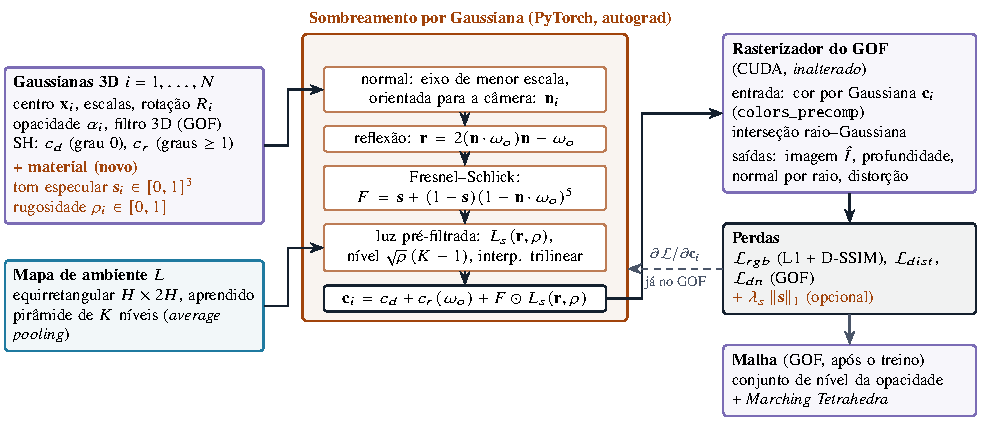
\includegraphics[width=\textwidth]{figuras/pipeline.pdf}
\caption{\textbf{Visão geral do método.}
O sombreamento (laranja) calcula, em PyTorch, uma cor $\bc_i$ por Gaussiana e por vista a partir dos atributos de material e de um mapa de ambiente aprendido.
Essa cor entra no rasterizador do GOF pelo caminho de cor pré-computada, que já existia e já devolvia $\partial\mathcal{L}/\partial\bc_i$; o restante do gradiente é obtido por diferenciação automática.
Rasterizador, perdas geométricas e extração de malha são os do GOF, sem modificação.}
\label{fig:pipeline}
\end{figure}

\subsection{Preliminares: renderização no GOF}
Cada Gaussiana $i$ tem centro $\mathbf{x}_i$, covariância $\Sigma_i=R_iS_iS_i^\top R_i^\top$ (rotação $R_i$ e escalas $S_i$), opacidade $\alpha_i$ e coeficientes SH de cor.
O GOF avalia, para cada raio de pixel, o valor máximo $\mathcal{G}_i$ da Gaussiana ao longo do raio (interseção raio--Gaussiana) e compõe as cores na ordem de profundidade~\cite{yu2024gof}:
\begin{equation}
C=\sum_{i} \bc_i\,\alpha_i\mathcal{G}_i\prod_{j<i}\left(1-\alpha_j\mathcal{G}_j\right).
\label{eq:composicao}
\end{equation}
No GOF, $\bc_i$ é a avaliação dos SH na direção da câmera para o centro da Gaussiana.
As mesmas quantidades produzem mapas de profundidade e de normal, usados em uma perda de distorção de profundidade e em uma perda de consistência entre a normal renderizada e a normal derivada da profundidade.
A superfície final é um conjunto de nível do campo de opacidade, extraído por \emph{Marching Tetrahedra}.
Nada disso é alterado neste trabalho: mudamos apenas o valor de $\bc_i$ na Eq.~\ref{eq:composicao}.

\subsection{Função de sombreamento}
Seguindo o GaussianShader~\cite{jiang2024gaussianshader}, cada Gaussiana recebe um tom especular $\bs_i\in[0,1]^3$ e uma rugosidade $\rho_i\in[0,1]$ (ambos parametrizados por sigmoide e inicializados em 0,05 e 0,70, isto é, um material quase difuso).
Sendo $\omega_o$ a direção unitária do centro da Gaussiana para a câmera, a cor é
\begin{equation}
\bc_i(\omega_o)=\max\!\Big(\underbrace{c_{d,i}+c_{r,i}(\omega_o)}_{\text{SH do GOF}}\;+\;F(\bn_i\!\cdot\!\omega_o,\bs_i)\odot L_s(\br_i,\rho_i),\;0\Big).
\label{eq:sombreamento}
\end{equation}

\paragraph{Termos difuso e residual.}
Em vez de criar um tensor novo para a cor residual, reaproveitamos a expansão SH que cada Gaussiana do GOF já possui: o grau 0 é constante em $\omega_o$ e faz o papel do difuso $c_d$, e os graus $\geq 1$ formam a parte dependente da vista, $c_r$.
O GaussianShader trata $c_d$ e $c_r$ como termos separados, com $c_r$ em SH de terceira ordem~\cite{jiang2024gaussianshader}; nossa leitura é uma reinterpretação que mantém a memória e garante a equivalência da Seção~\ref{sec:equivalencia}.
\textbf{Em todos os experimentos deste artigo usamos SH de grau 0}, por restrição de memória da GPU de 6\,GB; portanto $c_r\equiv 0$ e a dependência da vista vem apenas do termo especular.

\paragraph{Normal.}
Como no GaussianShader e no GIR~\cite{jiang2024gaussianshader,shi2025gir}, a normal de sombreamento é o eixo de menor escala da Gaussiana, $\bn_i=R_i\,\mathbf{e}_k$ com $k=\arg\min_j S_{i,jj}$, com o sinal escolhido de modo que $\bn_i\cdot\omega_o>0$.
O resíduo aprendível de normal do GaussianShader está implementado mas desligado nos experimentos.
Note que essa normal é por Gaussiana, enquanto a normal do GOF é por raio; as duas coincidem quando a Gaussiana é achatada, regime que as perdas geométricas do GOF favorecem, mas não são a mesma quantidade (Seção~\ref{sec:limitacoes}).

\paragraph{Reflexão e Fresnel.}
A direção de consulta à iluminação é a reflexão $\br_i=2(\bn_i\cdot\omega_o)\bn_i-\omega_o$~\cite{verbin2022refnerf}.
O fator especular usa a aproximação de Schlick~\cite{schlick1994fresnel} com o tom especular no papel da refletância em incidência normal:
\begin{equation}
F(\cos\theta,\bs)=\bs+(\mathbf{1}-\bs)(1-\cos\theta)^5,\qquad \cos\theta=\bn\cdot\omega_o .
\label{eq:fresnel}
\end{equation}
Este termo não existe na equação do GaussianShader, em que o tom multiplica a luz diretamente~\cite{jiang2024gaussianshader}; ele é uma escolha nossa, que faz bordas em ângulo rasante refletirem mais.
Como $F\to 1$ em ângulo rasante qualquer que seja $\bs$, a equivalência exata com o GOF exige desligar o Fresnel (Seção~\ref{sec:equivalencia}).

\paragraph{Luz especular pré-filtrada.}
A iluminação é um mapa de ambiente equirretangular aprendível $L$ de $H\times 2H$ texels, inicializado em 0,5 com ruído gaussiano de desvio 0,02 (o ruído evita partir de uma iluminação uniforme, sob a qual a rugosidade não tem gradiente).
A cada passo construímos uma pirâmide de $K=6$ níveis por média $2\times 2$ (\emph{average pooling}) e lemos $L_s(\br,\rho)$ no nível contínuo $\ell=\sqrt{\rho}\,(K-1)$, com interpolação bilinear dentro do nível e linear entre níveis.
Isso é uma aproximação barata da pré-filtragem do \emph{split-sum}~\cite{karis2013ue4,munkberg2022nvdiffrec}: o filtro é uma caixa, não a convolução pelo lóbulo GGX~\cite{walter2007ggx} usada nesses trabalhos.
Uma consequência importante, discutida na Seção~\ref{sec:mecanismo}, é que $\rho$ indexa um nível de desfoque cuja largura angular depende de $H$, e não é uma rugosidade física calibrada.
As coordenadas $(u,v)$ do mapa vêm de $\operatorname{atan2}$ e $\arccos$ da direção $\br$; afastamos a direção dos polos por $\varepsilon=10^{-4}$, porque o gradiente dessas funções diverge exatamente nos polos e, num treino real, bastou uma Gaussiana perto de um polo para levar a perda a \texttt{NaN}.

\paragraph{Referencial da iluminação.}
Em todos os experimentos o mapa é fixo no referencial do mundo, que é o caso físico de uma câmera orbitando um objeto parado sob luz fixa.
A implementação também permite indexar o mapa pela reflexão em coordenadas da câmera, pensada para captura em mesa giratória; a justificativa está no Material Suplementar (Seção~\ref{sec:mesa}) e esse modo \emph{não} foi avaliado empiricamente.

\subsection{Integração sem alterar o rasterizador}
O rasterizador do GOF, herdado do 3DGS, aceita uma cor RGB por Gaussiana já calculada (\texttt{colors\_precomp}) no lugar dos SH e devolve o gradiente da perda em relação a essa cor.
Calculamos a Eq.~\ref{eq:sombreamento} em PyTorch e a entregamos por esse caminho (Figura~\ref{fig:pipeline}).
Todo o gradiente a jusante (tom, rugosidade, rotação e escalas pela normal, e o próprio mapa de ambiente) é obtido por diferenciação automática, sem derivadas escritas à mão e sem código CUDA novo.
O ramo especular é ligado a partir da iteração 3.000; antes disso o modelo renderiza como o GOF.

\subsection{Perdas}
A perda é a do GOF, $\mathcal{L}_{rgb}+\lambda_{dist}\mathcal{L}_{dist}+\lambda_{dn}\mathcal{L}_{dn}$, com $\mathcal{L}_{rgb}=0{,}8\,\mathcal{L}_1+0{,}2\,\mathcal{L}_{\text{D-SSIM}}$~\cite{kerbl2023gaussian}, $\lambda_{dist}=100$ e $\lambda_{dn}=0{,}05$, acrescida opcionalmente de uma esparsidade do tom especular, $\lambda_s\,\mathbb{E}_i\lVert\bs_i\rVert_1$.
Essa esparsidade codifica a hipótese de que poucas Gaussianas são especulares, útil para reduzir a ambiguidade entre albedo claro e reflexo em cenas foscas.
Ela não é a perda homônima do GaussianShader, que atua sobre a opacidade~\cite{jiang2024gaussianshader}.

\subsection{Equivalência verificável}
\label{sec:equivalencia}
Para que a diferença entre ``GOF'' e ``GOF com sombreamento'' meça apenas o termo especular, verificamos por teste automatizado, na GPU, duas igualdades:
(a) renderizar com as cores calculadas em PyTorch pelo caminho pré-computado coincide com renderizar pelos SH avaliados no CUDA do GOF; e
(b) com $\bs\approx 0$ e Fresnel desligado, a Eq.~\ref{eq:sombreamento} reproduz o GOF.
Nos dois casos a diferença máxima por pixel é menor que $10^{-5}$.
Um terceiro teste confirma que, com o Fresnel ligado, a igualdade (b) deixa de valer, como esperado pela Eq.~\ref{eq:fresnel}.
Esses testes fazem parte de uma suíte de 36 testes que passam na versão usada nos experimentos (Material Suplementar, Seção~\ref{sec:testes}).

%%%%%%%%%%%%%%%%%%%%%%%%%%%%%%%%%%%%%%%%%%%%%%%%%%%%%%%%%%%%%%%%%%%%%%%%%%%%%%%%
\section{Protocolo experimental}
\label{sec:protocolo}

\subsection{Desenho}
O desenho separa três comparações de natureza diferente.
\textbf{(C1) Efeito do termo especular:} GOF contra GOF+BRDF com o mesmo código e os mesmos hiperparâmetros, diferindo só pela ativação do sombreamento; é a única comparação causal no sentido estrito.
\textbf{(C2) Efeito da configuração:} GOF+BRDF com a configuração usada no Truck contra GOF+BRDF ajustado; mede o efeito conjunto de três hiperparâmetros alterados ao mesmo tempo.
\textbf{(C3) Comparação de sistemas:} GOF+BRDF ajustado contra GaussianShader; os dois diferem em código, primitiva, normal, iluminação e hiperparâmetros, e a comparação informa o desempenho relativo, não a causa.

\subsection{Dados}
\paragraph{Truck.}
Cena externa do Tanks and Temples~\cite{knapitsch2017tanks}, com 251 fotografias e poses estimadas por \emph{structure-from-motion}~\cite{schonberger2016colmap}.
Treinamos em resolução reduzida por 2 (978$\times$546) e usamos como teste uma a cada oito imagens (32 vistas), como no protocolo do 3DGS.
A inicialização usa os pontos esparsos do SfM.

\paragraph{NeRO Glossy Synthetic.}
Objetos sintéticos refletores renderizados sob iluminação de ambiente real~\cite{liu2023nero}.
Escolhemos três dos oito objetos para caber no orçamento de GPU (cada treino leva de 2 a 6\,h), cobrindo do quase espelho ao material mais difuso: \emph{bell} (metal dourado quase espelhado), \emph{teapot} (metal prateado com curvatura variada) e \emph{cat} (corpo perolado sobre base metálica).
Usamos a divisão oficial em 96 vistas de treino e 32 de teste, a 800$\times$800, com o canal alfa composto sobre fundo branco.
Os dados foram convertidos pelo script do GaussianShader e, para o GOF, acrescentamos o campo de abertura horizontal da câmera exigido pelo leitor de cenas.
Os dois métodos partem de 100 mil pontos aleatórios.
Verificamos que as imagens de referência gravadas pelos dois métodos são idênticas pixel a pixel.

\subsection{Configurações}
A Tabela~\ref{tab:configs} lista as configurações.
Todas as variantes do GOF usam SH de grau 0, 30 mil iterações e o mesmo código; o GaussianShader usa o comando indicado no repositório dos autores para cenas sintéticas.

\begin{table}[t]
\centering
\caption{\textbf{Configurações avaliadas.} Hiperparâmetros não listados seguem os valores-padrão do GOF. O GaussianShader usa \texttt{-{}-brdf\_dim 0 -{}-sh\_degree -1 -{}-lambda\_predicted\_normal 2e-1 -{}-brdf\_env 512}, como no repositório dos autores, com iluminação em \emph{cubemap} e regras próprias para normal e ativação dos termos.}
\label{tab:configs}
\footnotesize
\linespread{1.0}\selectfont
\resizebox{\textwidth}{!}{%
\begin{tabular}{lcccc}
\toprule
 & GOF & GOF+BRDF (config. Truck) & GOF+BRDF ajustado & GaussianShader \\
\midrule
Sombreamento especular & não & sim & sim & sim \\
Mapa de ambiente & — & 128$\times$256 & 512$\times$1024 & \emph{cubemap} $6\times512^2$ \\
Esparsidade do tom $\lambda_s$ & — & 0,001 & 0 & — \\
Consistência de normal a partir de & 15.000 & 15.000 & 3.000 & (própria) \\
Especular a partir de & — & 3.000 & 3.000 & (própria) \\
Fresnel--Schlick & — & sim & sim & não \\
Grau SH da cor & 0 & 0 & 0 & $-1$ (cor pelo ramo BRDF) \\
Iterações & 30.000 & 30.000 & 30.000 & 30.000 \\
\bottomrule
\end{tabular}}
\end{table}

\paragraph{Como o ajuste foi escolhido.}
Com a configuração do Truck, o GOF+BRDF ficou 5\dB{} abaixo do GaussianShader na \emph{bell}.
O diagnóstico apontou quatro causas possíveis: rugosidade aprendida alta num objeto espelhado, mapa de ambiente de baixa resolução, esparsidade empurrando o tom especular para zero e regularização de normal iniciada tarde (15 mil iterações) em relação ao ramo especular (3 mil).
As três últimas foram alteradas juntas e conferidas em treinos curtos de 7.002 iterações na \emph{bell}, com PSNR do avaliador interno de 23,75 (GOF), 24,36 (config. Truck) e 27,44\dB{} (ajustado), antes dos treinos completos nas três cenas.
Como a \emph{bell} é também cena de teste, o ganho nela está sujeito a viés de seleção; \emph{cat} e \emph{teapot} não participaram da escolha e funcionam como evidência fora da amostra para o ajuste.
A primeira causa foi testada depois, pelas distribuições de material (Seção~\ref{sec:mecanismo}), e não se confirmou.

\subsection{Métricas}
Medimos PSNR, SSIM~\cite{wang2004ssim} e LPIPS com rede VGG~\cite{zhang2018lpips} sobre as imagens de teste gravadas por cada método, com o mesmo código para todos (a implementação de métricas do GOF), na imagem inteira.
No NeRO o fundo branco entra no cálculo e eleva os valores absolutos de todos os métodos por igual; as comparações são relativas.

\subsection{Análise estatística}
A unidade de análise é a vista de teste.
Para cada par de métodos calculamos a diferença por vista e reportamos a média, um intervalo de confiança de 95\% por \emph{bootstrap} pareado das diferenças (10 mil reamostragens)~\cite{efron1979bootstrap}, o valor-$p$ bilateral do teste de postos sinalizados de Wilcoxon~\cite{wilcoxon1945}, o tamanho de efeito $d_z$ de Cohen e o número de vistas em que cada método é melhor.
Com 32 vistas e todas as diferenças do mesmo sinal, o menor $p$ possível do teste exato é $2/2^{32}\approx4{,}7\times10^{-10}$.
Ao todo reportamos 24 pares em 3 métricas (72 testes); o limiar de Bonferroni para $\alpha=0{,}05$ seria $6{,}9\times10^{-4}$, e todas as diferenças que tratamos como significativas têm $p\leq1{,}0\times10^{-4}$; os dois efeitos que tratamos como nulos são o PSNR da \emph{bell} em C1 ($p=0{,}59$) e em C3 ($p=0{,}71$).

Essa análise trata cada modelo treinado como fixo: o intervalo descreve a incerteza devida à amostra de vistas, não a variação entre treinos.
O treino do GOF não é reprodutível bit a bit, porque o rasterizador acumula gradientes com operações atômicas cuja ordem varia; por isso, com uma semente por configuração, consideramos não interpretáveis diferenças médias de PSNR abaixo de cerca de 0,1\dB, mesmo quando o intervalo exclui o zero.

\subsection{Custo}
Todos os treinos rodaram um por vez na mesma máquina, com uma GPU NVIDIA RTX 3050 de 6\,GB (CUDA 11.8, PyTorch 2.0.1); o GaussianShader rodou em ambiente separado, conforme seu repositório.
No NeRO, um processo auxiliar amostrou o \texttt{nvidia-smi} a cada 2\,s durante o treino.
Reportamos o tempo de parede do treino, a potência média da placa, a energia como potência média vezes tempo (apenas a GPU, sem CPU nem fonte; ver~\cite{strubell2019energy} sobre a importância de reportar esse custo) e a memória de vídeo máxima ocupada segundo o \texttt{nvidia-smi}, que inclui o cache do alocador e o contexto CUDA e é, portanto, um limite superior da memória necessária.
No Truck, medido antes desse instrumento, reportamos o tempo de parede dos registros de treino e o pico de memória alocada pelo PyTorch, que é outra medida e não deve ser comparada diretamente com a do NeRO.

%%%%%%%%%%%%%%%%%%%%%%%%%%%%%%%%%%%%%%%%%%%%%%%%%%%%%%%%%%%%%%%%%%%%%%%%%%%%%%%%
\section{Resultados}
\label{sec:resultados}

\subsection{Cena real: Truck}
A Tabela~\ref{tab:truck} mostra a comparação controlada C1 no Truck.
O termo especular aumenta o PSNR em 0,41\dB{} (IC 95\%: +0,29 a +0,53), com ganho em 28 das 32 vistas, e aumenta o SSIM em todas as vistas.
O LPIPS, ao contrário, piora levemente (+0,0025) em 30 das 32 vistas.
O ganho é distribuído pelas vistas (mediana +0,38\dB); o maior é de 1,66\dB, na vista mostrada na Figura~\ref{fig:truck}, e nas quatro vistas em que o GOF fica à frente a diferença não passa de 0,14\dB.
Na vista de maior ganho, a redução do erro não se concentra numa região especular: no terço superior, no meio e na parte de baixo da imagem, o GOF+BRDF erra menos em 56 a 58\% dos pixels, e há também regiões em que o erro aumenta, como uma mancha no chão à direita (Figura~\ref{fig:truck}).
O número de Gaussianas finais é praticamente o mesmo (2,09 e 2,08 milhões), o tempo de treino passa de 6\,h\,51\,min para 8\,h\,22\,min (+22\%), e o pico de memória alocada do GOF+BRDF foi de 3,99\,GB (no GOF, cerca de 2,9\,GB, medido até a iteração 6.777).
Para comparação, o GaussianShader relata ganho médio de +0,19\dB{} sobre o 3DGS no Tanks and Temples, cujos objetos são predominantemente difusos, e de +0,04\dB{} no próprio Truck (Tabela 6 de~\cite{jiang2024gaussianshader}); o efeito que medimos é maior, mas a comparação entre trabalhos não é direta, porque a base (3DGS ou GOF), a resolução e o protocolo diferem.
Comparações no Truck com o GaussianShader e com outra configuração do GOF, treinados em outra máquina e com outros hiperparâmetros, estão na Tabela~\ref{tab:truck_externos} e não são controladas.

\begin{table}[t]
\centering
\caption{\textbf{Truck: efeito do termo especular (C1).} Média das 32 vistas de teste, uma semente por configuração. $\Delta$ = GOF+BRDF $-$ GOF; para o LPIPS, menor é melhor.}
\label{tab:truck}
\footnotesize
\linespread{1.0}\selectfont
\begin{tabular}{lccc}
\toprule
 & PSNR (dB) $\uparrow$ & SSIM $\uparrow$ & LPIPS $\downarrow$ \\
\midrule
\inputtab{tabelas/truck.tex}
\bottomrule
\end{tabular}
\end{table}

\begin{figure}[t]
\centering
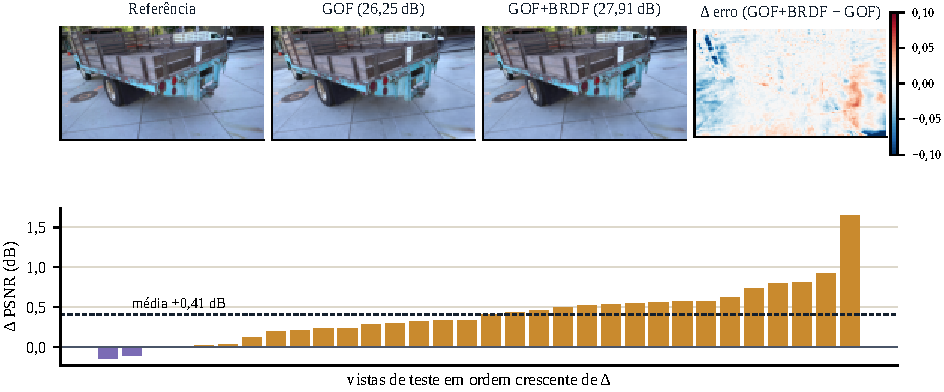
\includegraphics[width=\textwidth]{figuras/truck.pdf}
\caption{\textbf{Truck.} Acima: vista de teste com o maior ganho do termo especular (vista 24), e a diferença do erro absoluto por pixel, GOF+BRDF menos GOF (azul: o GOF+BRDF erra menos). Abaixo: diferença de PSNR por vista, ordenada; a linha tracejada é a média.}
\label{fig:truck}
\end{figure}

\subsection{Objetos brilhantes: NeRO}
A Tabela~\ref{tab:nero} e a Figura~\ref{fig:nero_metricas} trazem as métricas médias; a Tabela~\ref{tab:pares} e a Figura~\ref{fig:efeitos}, as diferenças pareadas.

\paragraph{C1, termo especular com a configuração do Truck.}
No \emph{cat} e no \emph{teapot} o termo especular rende +2,49\dB{} (IC: +2,27 a +2,69) e +2,00\dB{} (+1,61 a +2,40) sobre o GOF, com SSIM e LPIPS também melhores.
Na \emph{bell}, o objeto mais espelhado, o efeito em PSNR é nulo ($-$0,04\dB{}; IC $-$0,26 a +0,18; $p=0{,}59$), e SSIM e LPIPS pioram levemente.

\paragraph{C2, efeito do ajuste.}
O ajuste soma +5,02\dB{} na \emph{bell}, +0,32\dB{} no \emph{cat} e +1,33\dB{} no \emph{teapot}, com as três métricas melhores nas três cenas.
O ganho no \emph{cat} e no \emph{teapot}, que não participaram da escolha, indica que o ajuste não é específico da \emph{bell}, embora seja muito menor fora dela.

\paragraph{C3, comparação com o GaussianShader.}
Na \emph{bell}, os dois empatam em PSNR ($-$0,01\dB; IC $-$0,24 a +0,23; $p=0{,}71$; o GOF+BRDF ajustado é melhor em 17 das 32 vistas), mas o GaussianShader tem SSIM (+0,0055) e LPIPS ($-$0,0033) significativamente melhores.
No \emph{cat} e no \emph{teapot}, o GOF+BRDF ajustado é melhor nas três métricas, com PSNR maior em todas as 32 vistas (+1,37 e +0,58\dB).
Para verificar que o GaussianShader não foi prejudicado pela nossa execução, comparamos com os valores publicados pelos autores para os mesmos objetos (linhas em itálico na Tabela~\ref{tab:nero}): nossa execução fica 1,76\dB{} acima do publicado na \emph{bell}, 0,25\dB{} acima no \emph{teapot} e 0,49\dB{} abaixo no \emph{cat}.

\paragraph{Inspeção visual.}
Na Figura~\ref{fig:nero_qualitativo}, o erro se concentra nos reflexos do ambiente.
Na \emph{bell}, sem ajuste, o ambiente refletido vira manchas com ou sem o termo especular; com o ajuste, os contornos do reflexo aparecem, como no GaussianShader.
Sem o termo especular, o metal do \emph{teapot} perde contraste e o \emph{cat} perde o brilho perolado.

\begin{table}[t]
\centering
\caption{\textbf{NeRO: métricas médias nas 32 vistas de teste.} Negrito: melhor média da cena (na \emph{bell}, a diferença de PSNR entre o GOF+BRDF ajustado e o GaussianShader não é significativa; Tabela~\ref{tab:pares}). Itálico: valores publicados pelos autores do GaussianShader para o mesmo objeto (Tabela 5 de~\cite{jiang2024gaussianshader}), como referência da nossa execução.}
\label{tab:nero}
\footnotesize
\linespread{1.0}\selectfont
\begin{tabular}{llccc}
\toprule
Cena & Método & PSNR (dB) $\uparrow$ & SSIM $\uparrow$ & LPIPS $\downarrow$ \\
\midrule
\inputtab{tabelas/nero_metricas.tex}
\bottomrule
\end{tabular}
\end{table}

\begin{table}[t]
\centering
\caption{\textbf{NeRO: diferenças pareadas por vista.} Média e IC 95\% por \emph{bootstrap} pareado; $p$ do teste de Wilcoxon para o PSNR; última coluna: vistas em que o primeiro termo tem PSNR maior. Diferenças positivas favorecem o primeiro termo em PSNR e SSIM, e negativas em LPIPS. Estatísticas de todos os pares estão na Tabela~\ref{tab:pares_completa}.}
\label{tab:pares}
\scriptsize
\linespread{1.0}\selectfont
\resizebox{\textwidth}{!}{%
\begin{tabular}{llccccc}
\toprule
Cena & Contraste & $\Delta$PSNR (dB) & $\Delta$SSIM & $\Delta$LPIPS & $p$ (PSNR) & vistas \\
\midrule
\inputtab{tabelas/nero_pares.tex}
\bottomrule
\end{tabular}}
\end{table}

\begin{figure}[p]
\centering
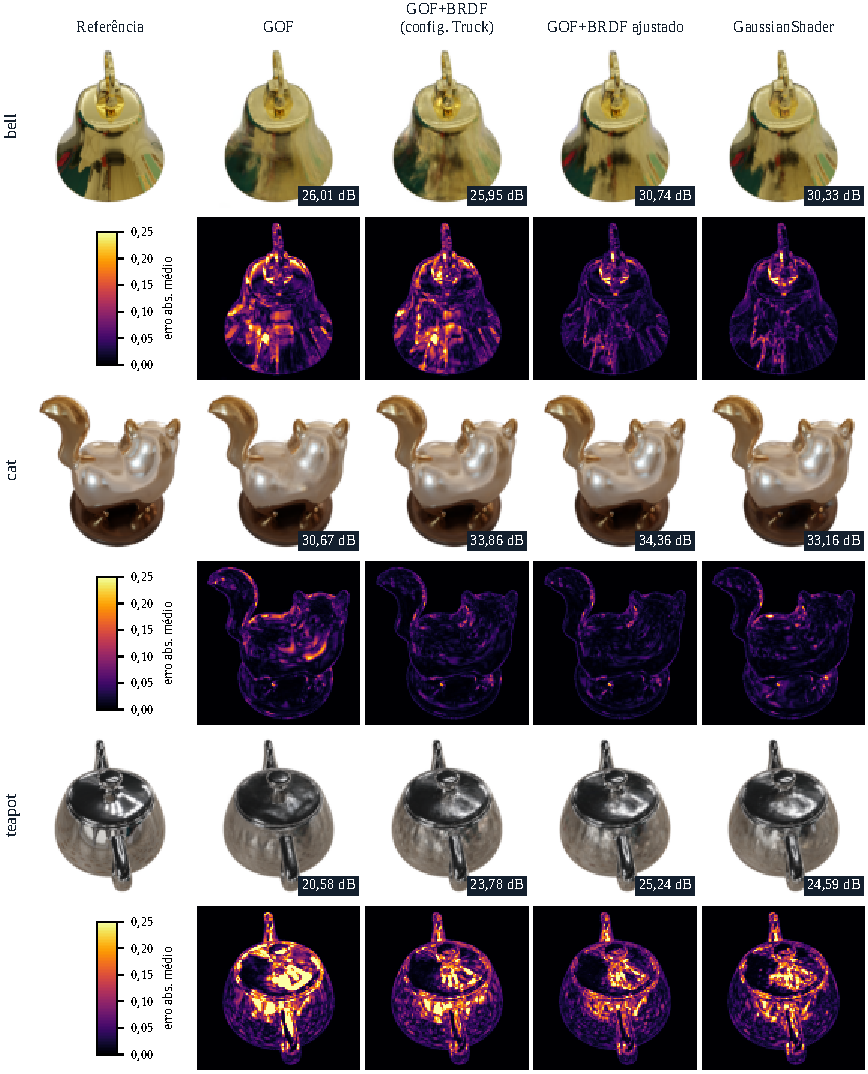
\includegraphics[width=\textwidth]{figuras/nero_qualitativo.pdf}
\caption{\textbf{NeRO, vista de teste 5 de cada objeto.} Linhas ímpares: referência e renders, com o PSNR da vista; linhas pares: erro absoluto médio por pixel, na mesma escala para todos os métodos.}
\label{fig:nero_qualitativo}
\end{figure}

\begin{figure}[t]
\centering
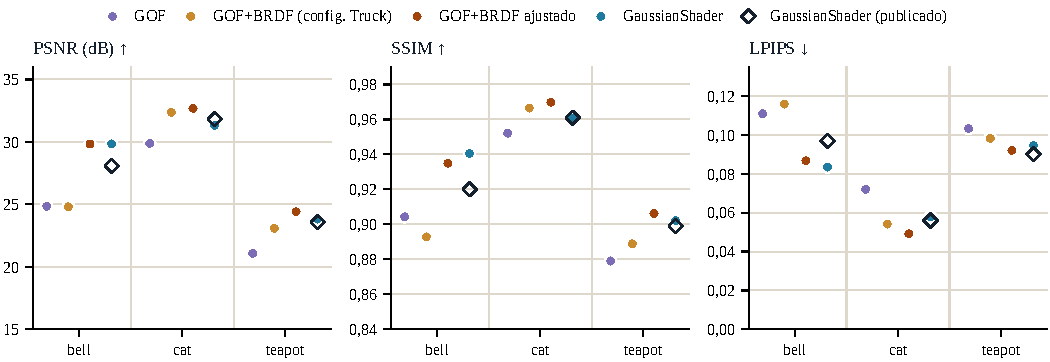
\includegraphics[width=\textwidth]{figuras/nero_metricas.pdf}
\caption{\textbf{NeRO: métricas médias por objeto.} Os losangos vazados são os valores publicados para o GaussianShader~\cite{jiang2024gaussianshader}; os eixos verticais não começam em zero.}
\label{fig:nero_metricas}
\end{figure}

\begin{figure}[t]
\centering
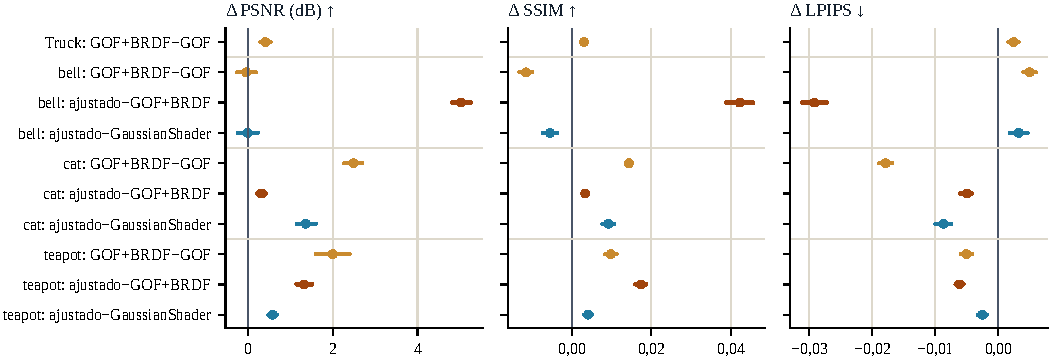
\includegraphics[width=\textwidth]{figuras/efeitos_pareados.pdf}
\caption{\textbf{Efeitos pareados com intervalo de confiança de 95\%.} Cada linha é um contraste: termo especular com a mesma configuração (laranja-claro, incluindo o Truck), efeito do ajuste (laranja-escuro) e GOF+BRDF ajustado menos GaussianShader (azul). Para o LPIPS, valores negativos favorecem o primeiro termo.}
\label{fig:efeitos}
\end{figure}

\subsection{Custo}
A Tabela~\ref{tab:custo} e a Figura~\ref{fig:custo} mostram o custo de treino.
Em relação ao GOF+BRDF ajustado, o GaussianShader leva de 1,9 a 3,0 vezes o tempo, gasta de 2,7 a 4,0 vezes a energia da GPU (potência média de 68\,W contra cerca de 49\,W) e ocupa cerca do dobro da memória, perto do limite de 6\,GB da placa.
O GaussianShader termina com 2,0 a 2,7 vezes mais Gaussianas.
O ajuste não encarece o treino: tempo e energia do GOF+BRDF ajustado ficam iguais ou menores que os da configuração do Truck, e a memória fica entre 2,6 e 2,7\,GB.
A renderização das 32 vistas de teste, incluindo carga do modelo e gravação das imagens, leva cerca de 20 a 24\,s nas variantes do GOF e 50 a 52\,s no GaussianShader; esse tempo não é uma medida de quadros por segundo.
A potência ao longo do treino está na Figura~\ref{fig:potencia}.

\begin{table}[t]
\centering
\caption{\textbf{NeRO: custo do treino de 30 mil iterações na RTX 3050 (6\,GB).} Energia = potência média da GPU $\times$ tempo; memória = máximo do \texttt{nvidia-smi}; Gaussianas ao final do treino; render = tempo de parede para renderizar as 32 vistas de teste.}
\label{tab:custo}
\footnotesize
\linespread{1.0}\selectfont
\resizebox{\textwidth}{!}{%
\begin{tabular}{llcccccc}
\toprule
Cena & Método & Tempo (h) & Energia (Wh) & Potência (W) & Memória (GB) & Gaussianas (mil) & Render (s) \\
\midrule
\inputtab{tabelas/custo.tex}
\bottomrule
\end{tabular}}
\end{table}

\begin{figure}[t]
\centering
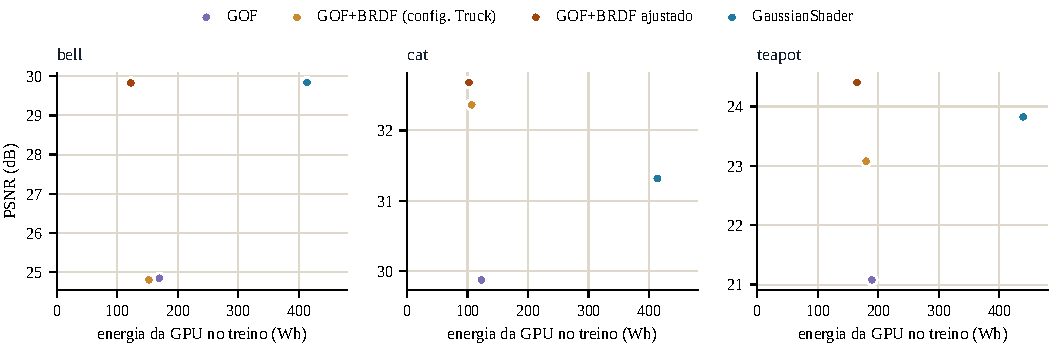
\includegraphics[width=\textwidth]{figuras/custo_qualidade.pdf}
\caption{\textbf{Qualidade contra energia de treino no NeRO.} Cada ponto é um treino completo.}
\label{fig:custo}
\end{figure}

\subsection{Por que a configuração importa}
\label{sec:mecanismo}
O diagnóstico inicial da \emph{bell} incluía a hipótese de que o modelo aprendia uma rugosidade alta demais para um objeto espelhado.
As distribuições de material aprendidas (Tabela~\ref{tab:material} e Figura~\ref{fig:mecanismo}) não sustentam essa hipótese: com o ajuste, a rugosidade mediana fica igual na \emph{bell} (0,54 e 0,56) e \emph{aumenta} no \emph{cat} e no \emph{teapot}.
O que muda de forma consistente nas três cenas é o tom especular: a mediana passa de 0,12--0,23 para 0,32--0,57, e a fração de Gaussianas com tom acima de 0,1, ponderada pela opacidade, passa de 54--66\% para 77--84\%.
Isso é o esperado ao remover a esparsidade do tom, que penaliza exatamente essa grandeza.

A resolução do mapa explica por que a mesma rugosidade pode produzir reflexos muito mais nítidos.
O nível lido é $\ell=\sqrt{\rho}\,(K-1)$, e um nível $\ell$ de um mapa de altura $H$ tem $H/2^{\ell}$ texels para 180$^\circ$.
Para $\rho=0{,}56$ e $K=6$, $\ell\approx3{,}7$: o texel tem cerca de 19$^\circ$ com $H=128$ e cerca de 4,7$^\circ$ com $H=512$.
Ou seja, nesta formulação $\rho$ não é uma rugosidade física, mas um índice de desfoque cuja largura angular é proporcional a $1/H$; valores de $\rho$ não são comparáveis entre configurações com $H$ diferente.
Os mapas aprendidos na \emph{bell} (Figura~\ref{fig:mecanismo}, abaixo) são coerentes com essa leitura: com $H=512$ o mapa mostra uma estrutura de ambiente reconhecível, e com $H=128$ apenas blocos.
Como os três ajustes foram aplicados juntos, esses dados indicam mecanismos plausíveis, mas não medem a contribuição de cada ajuste.

\begin{table}[t]
\centering
\caption{\textbf{Material aprendido pelo GOF+BRDF no NeRO.} Estatísticas ponderadas pela opacidade das Gaussianas; tom = média dos três canais; rugosidade com mediana e quartis.}
\label{tab:material}
\footnotesize
\linespread{1.0}\selectfont
\begin{tabular}{llccc}
\toprule
Cena & Configuração & Tom mediano & Tom $>0{,}1$ & Rugosidade mediana [Q1; Q3] \\
\midrule
\inputtab{tabelas/material.tex}
\bottomrule
\end{tabular}
\end{table}

\begin{figure}[t]
\centering
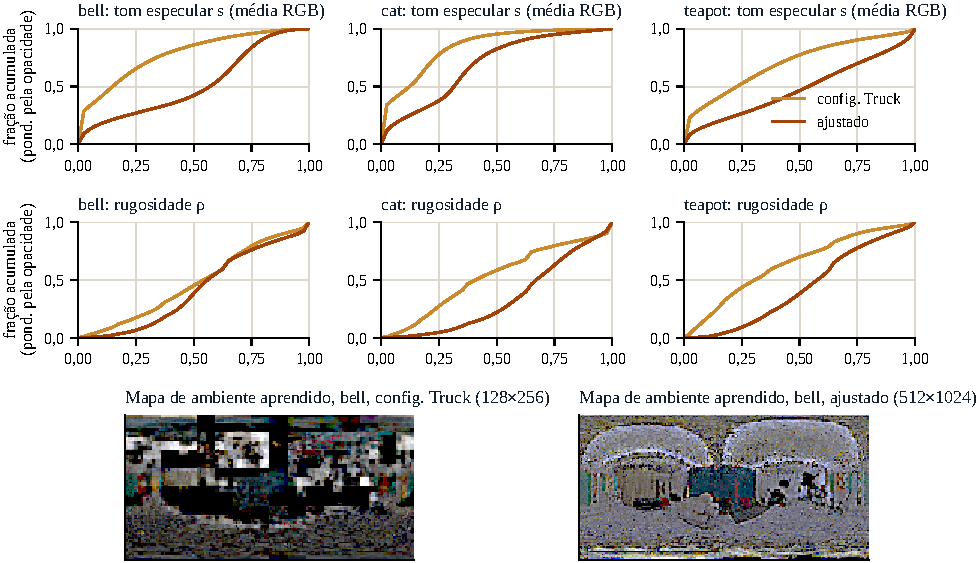
\includegraphics[width=\textwidth]{figuras/mecanismo.pdf}
\caption{\textbf{Mecanismo do ajuste.} Distribuições acumuladas, ponderadas pela opacidade, do tom especular (primeira linha) e da rugosidade (segunda linha), para a configuração do Truck e a ajustada. Abaixo: mapa de ambiente aprendido na \emph{bell} em cada configuração (exibição com escala no percentil 99,5 e gama 2,2).}
\label{fig:mecanismo}
\end{figure}

%%%%%%%%%%%%%%%%%%%%%%%%%%%%%%%%%%%%%%%%%%%%%%%%%%%%%%%%%%%%%%%%%%%%%%%%%%%%%%%%
\section{Discussão}

\paragraph{Respostas à pergunta de pesquisa.}
(i) A integração reproduz o GOF quando o termo especular é nulo e o Fresnel está desligado, o que é verificado por teste e torna a comparação C1 interpretável.
(ii) O termo especular melhora a síntese de vistas no Truck (+0,41\dB) e em dois dos três objetos com a configuração herdada; no objeto mais espelhado, ele só passa a ajudar depois do ajuste.
(iii) Com o ajuste, o GOF+BRDF empata com o GaussianShader em PSNR na \emph{bell}, com SSIM e LPIPS um pouco piores, e o supera nas três métricas no \emph{cat} e no \emph{teapot}, com menos tempo, energia e memória.

\paragraph{A configuração pode anular o termo especular.}
O achado mais útil na prática é que a mesma formulação vai de ``nenhum ganho'' a ``empate com o GaussianShader'' na \emph{bell} mudando hiperparâmetros pensados para cenas foscas.
A esparsidade do tom é razoável quando poucas superfícies são especulares, mas num objeto metálico ela empurra o tom justamente para o valor que desliga o reflexo; e um mapa de 128 texels de altura limita a nitidez do reflexo qualquer que seja a rugosidade aprendida.
Isso sugere tratar esses hiperparâmetros como dependentes da classe de material da cena, e não como constantes do método.

\paragraph{Por que o GOF+BRDF pode superar o GaussianShader.}
Não testamos a causa da vantagem no \emph{cat} e no \emph{teapot}.
Hipóteses compatíveis com os dados são a renderização por interseção raio--Gaussiana e as perdas geométricas do GOF, que poderiam dar normais mais estáveis ao termo especular, e o Fresnel, ausente no GaussianShader.
O GaussianShader termina com cerca do dobro de Gaussianas, o que torna improvável que a diferença venha de falta de capacidade do GaussianShader.
Separar essas causas exigiria ablações cruzadas que não fizemos.

\paragraph{Discordância entre métricas.}
No Truck, PSNR e SSIM favorecem o GOF+BRDF e o LPIPS favorece o GOF; na \emph{bell} (C3), o PSNR empata e SSIM e LPIPS favorecem o GaussianShader.
O LPIPS mede semelhança de características profundas e pode penalizar padrões de alta frequência que o PSNR quase não vê; diferenças de LPIPS da ordem de 0,003 são pequenas, mas, sendo consistentes entre vistas, não devem ser descartadas.

\paragraph{Relação com a literatura.}
O resultado é coerente com a observação de que o ganho de modelos de sombreamento cresce com a especularidade da cena~\cite{jiang2024gaussianshader}.
Ele não toca as questões abertas da terceira onda de trabalhos, como iluminação indireta, visibilidade e reconstrução de material com significado físico~\cite{gu2025irgs,zhu2026ptirgs,han2026radiometric}; nosso método ignora essas componentes por construção.

\subsection{Ameaças à validade}
\paragraph{Validade interna.}
Há uma semente por configuração, e o treino não é reprodutível bit a bit; os intervalos de confiança cobrem a variação entre vistas, não entre treinos.
O ajuste foi escolhido na \emph{bell}, que também é cena de teste.
Os três ajustes foram aplicados juntos.
O esforço de ajuste foi assimétrico: ajustamos o nosso método e usamos o GaussianShader na configuração dos autores; o fato de nossa execução do GaussianShader ficar acima do publicado em dois dos três objetos atenua, mas não elimina, essa ameaça.
\paragraph{Validade externa.}
Avaliamos uma cena real e três objetos sintéticos, todos com iluminação fixa no mundo.
Não avaliamos geometria, relighting nem a qualidade do material recuperado, e o modo de iluminação em referencial de câmera não foi testado.
\paragraph{Validade de construto.}
As métricas incluem o fundo branco no NeRO; a energia é só a da GPU; a memória do NeRO vem do \texttt{nvidia-smi} e inclui reservas do alocador; o tempo de render inclui leitura e escrita de arquivos.

\section{Limitações e trabalhos futuros}
\label{sec:limitacoes}
\emph{Sombreamento por Gaussiana.} A cor é avaliada uma vez por Gaussiana e por vista, como no GaussianShader; um reflexo menor que uma Gaussiana não pode ser representado, e a normal usada não é a normal por raio do GOF.
Um sombreamento por pixel com a normal por raio exigiria alterar o rasterizador.
\emph{Sem luz indireta, sem visibilidade.} Inter-reflexões e sombras ficam por conta do mapa de ambiente e do difuso.
\emph{Rugosidade não identificável e não calibrada.} Sob iluminação uniforme, $\partial\mathcal{L}/\partial\rho=0$; e, com a pirâmide por média, $\rho$ depende de $H$ (Seção~\ref{sec:mecanismo}).
\emph{Memória.} Em 6\,GB usamos SH de grau 0, o que desliga o termo residual; graus maiores não foram medidos.
\emph{Geometria.} A extração de malha de cenas com cerca de 2 milhões de Gaussianas não coube em 6\,GB na implementação original; um processamento em lotes está em desenvolvimento, e métricas de geometria (Chamfer, F1) ficam para a próxima versão.
\emph{Próximos passos.} Repetir os treinos com ao menos três sementes; separar os três ajustes por ablação; avaliar os outros cinco objetos do NeRO e a geometria contra as malhas de referência; e validar o modo em referencial de câmera numa captura em mesa giratória.
A motivação original deste estudo é a documentação digital de amostras com microestruturas brilhantes, como testemunhos de sondagem, cuja avaliação depende de autorização de uso dos dados.

\section{Conclusão}
Acoplar o sombreamento especular do GaussianShader ao GOF pelo caminho de cor pré-computada é suficiente para dar ao GOF um termo especular útil, sem alterar o rasterizador nem a extração de malha, e com equivalência verificável ao GOF.
O ganho é pequeno numa cena real predominantemente fosca e grande em objetos brilhantes, desde que a configuração não neutralize o termo especular; ajustado, o método iguala ou supera o GaussianShader nos três objetos testados em PSNR, com uma fração da energia e da memória.
Esses números vêm de uma semente por configuração e de um ajuste escolhido em uma das cenas de teste, e devem ser lidos como evidência preliminar até a repetição com várias sementes e a ablação dos ajustes.

\section*{Disponibilidade de código e dados}
O código, os scripts de treino, medição de custo, métricas e estatística, e os scripts que geram todas as figuras e tabelas deste manuscrito a partir dos resultados estão em \revisar{repositório a definir}.
Os dados usados são públicos~\cite{knapitsch2017tanks,liu2023nero}.

\section*{Agradecimentos}
\revisar{Preencher: financiamento, infraestrutura, contribuições de cada autor.}

\bibliographystyle{sciencemag}
\bibliography{referencias}

%%%%%%%%%%%%%%%%%%%%%%%%%%%%%%%%%%%%%%%%%%%%%%%%%%%%%%%%%%%%%%%%%%%%%%%%%%%%%%%%
\newpage
\renewcommand{\thefigure}{S\arabic{figure}}
\renewcommand{\thetable}{S\arabic{table}}
\renewcommand{\theequation}{S\arabic{equation}}
\renewcommand{\thesection}{S\arabic{section}}
\setcounter{figure}{0}
\setcounter{table}{0}
\setcounter{equation}{0}
\setcounter{section}{0}

\begin{center}
\section*{Material Suplementar}
\end{center}

\section{Comparações adicionais no Truck}
A Tabela~\ref{tab:truck_externos} inclui dois sistemas treinados em outra máquina, com outros hiperparâmetros: o GaussianShader com sua configuração própria e o GOF com SH de grau 3 e aparência desacoplada.
As imagens de referência das três origens são idênticas pixel a pixel, mas as diferenças de configuração impedem atribuir causa às diferenças entre esses sistemas e os nossos.

\begin{table}[h]
\centering
\caption{\textbf{Truck: comparação não controlada.} $^\dagger$Treinado em outra máquina, com hiperparâmetros próprios; não comparável de forma causal.}
\label{tab:truck_externos}
\footnotesize
\linespread{1.0}\selectfont
\begin{tabular}{lccc}
\toprule
Sistema & PSNR (dB) $\uparrow$ & SSIM $\uparrow$ & LPIPS $\downarrow$ \\
\midrule
\inputtab{tabelas/truck_externos.tex}
\bottomrule
\end{tabular}
\end{table}

\section{Estatísticas completas do NeRO}
\begin{table}[h]
\centering
\caption{\textbf{NeRO: todos os pares.} Média [IC 95\%] da diferença ``primeiro $-$ segundo''; $p$ de Wilcoxon para o PSNR (os de SSIM e LPIPS estão em \texttt{dados/nero/*\_analysis.json}).}
\label{tab:pares_completa}
\scriptsize
\linespread{1.0}\selectfont
\resizebox{\textwidth}{!}{%
\begin{tabular}{llcccc}
\toprule
Cena & Par & $\Delta$PSNR (dB) & $\Delta$SSIM & $\Delta$LPIPS & $p$ (PSNR) \\
\midrule
\inputtab{tabelas/nero_pares_completa.tex}
\bottomrule
\end{tabular}}
\end{table}

\begin{figure}[h]
\centering
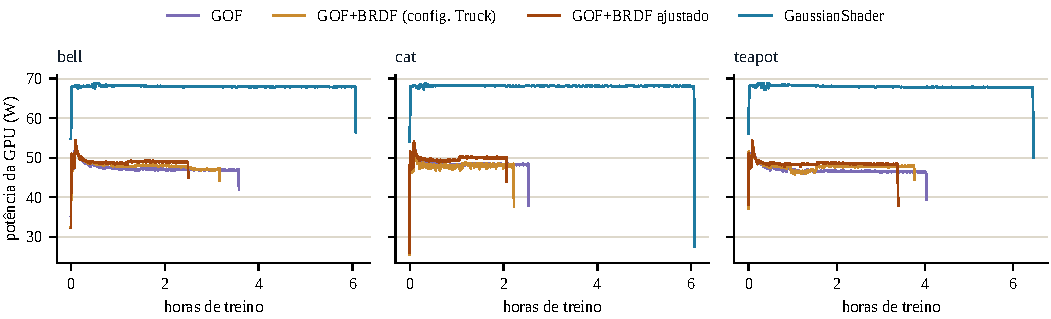
\includegraphics[width=\textwidth]{figuras/potencia.pdf}
\caption{\textbf{Potência da GPU ao longo do treino} (média móvel das amostras de 2\,s).}
\label{fig:potencia}
\end{figure}

\begin{figure}[h]
\centering
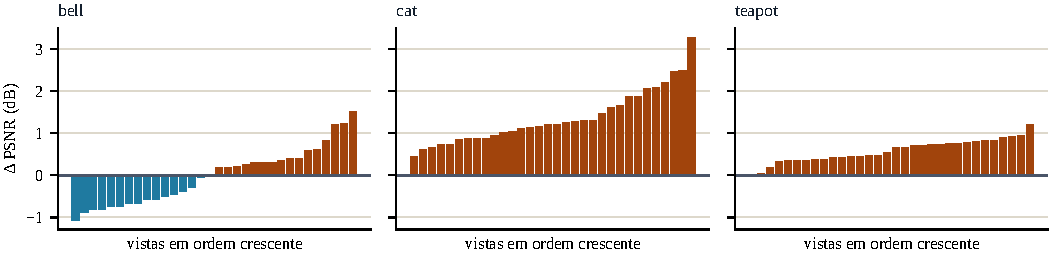
\includegraphics[width=\textwidth]{figuras/por_vista_ajustado_gs.pdf}
\caption{\textbf{Diferença de PSNR por vista, GOF+BRDF ajustado menos GaussianShader}, ordenada (laranja: GOF+BRDF ajustado melhor; azul: GaussianShader melhor).}
\label{fig:por_vista}
\end{figure}

\section{Testes e modos de falha silenciosos}
\label{sec:testes}
A suíte automatizada tem 36 testes, executados na GPU, que passam na versão usada nos experimentos.
Além das igualdades da Seção~\ref{sec:equivalencia}, ela cobre propriedades da reflexão (involução e preservação de norma), os limites do Fresnel (refletância $\bs$ em incidência normal e 1 em ângulo rasante), o efeito do referencial da iluminação e a orientação da normal.
Cinco falhas encontradas durante o desenvolvimento não geravam erro nem mudavam o formato dos tensores, e por isso só foram detectadas comparando o comportamento com o esperado; cada uma tem hoje um teste de regressão.
\begin{enumerate}
\item \emph{Material desvinculado do otimizador na poda.} Ao podar Gaussianas, o tensor de material era recriado a partir do valor antigo; o modelo passava a ler um tensor e o otimizador a atualizar outro, e o material congelava na primeira poda.
\item \emph{Material ausente do \emph{checkpoint}.} Retomar um treino recriava o material vazio.
\item \emph{Material ausente do arquivo de pontos final.} A avaliação, que recarrega o modelo desse arquivo, usaria material padrão, diferente do treinado.
\item \emph{Iluminação ausente do \emph{checkpoint}.} Retomar um treino reiniciaria o mapa de ambiente aprendido, mantendo o estado do otimizador calculado para o mapa antigo.
\item \emph{Gradiente infinito nos polos do mapa.} O primeiro treino real com o termo especular foi a \texttt{NaN} dez iterações após a ativação do ramo especular; a correção é o afastamento $\varepsilon$ da Seção~\ref{sec:metodo}.
\end{enumerate}

\section{Iluminação em referencial de câmera (não validada)}
\label{sec:mesa}
Numa mesa giratória, o objeto gira e a câmera e as luzes ficam paradas.
Sejam $R_i$ a rotação (desconhecida) da mesa na imagem $i$ e $C$ a rotação constante da sala para a câmera.
O \emph{structure-from-motion} vê o objeto parado e entrega a rotação mundo--câmera $W_i=C\,R_i$.
Uma direção de reflexão $\br_O$ em coordenadas do objeto corresponde, na sala, a
\begin{equation}
\br_{\text{sala}}=R_i\,\br_O=C^{-1}(C R_i)\,\br_O=C^{-1}W_i\,\br_O=C^{-1}\br_{\text{câm}},
\end{equation}
em que $\br_{\text{câm}}$ é a reflexão em coordenadas da câmera.
Portanto $L(\br_{\text{sala}})=L'(\br_{\text{câm}})$, com $L'=L\circ C^{-1}$: indexar um mapa aprendido pela reflexão em coordenadas da câmera equivale a aprender o mapa da sala pré-rotacionado por uma rotação global constante, sem estimar o ângulo da mesa.
A dedução exige que a orientação da câmera seja a mesma em todas as fotos (translações são permitidas); com várias orientações seria necessária uma rotação por estação.
Este modo está implementado, com um teste que verifica apenas que a rotação é aplicada; nenhum experimento deste artigo o utiliza.

\end{document}
